\documentclass{standalone}
\usepackage{tikz}
\usetikzlibrary{patterns, positioning}

\begin{document}
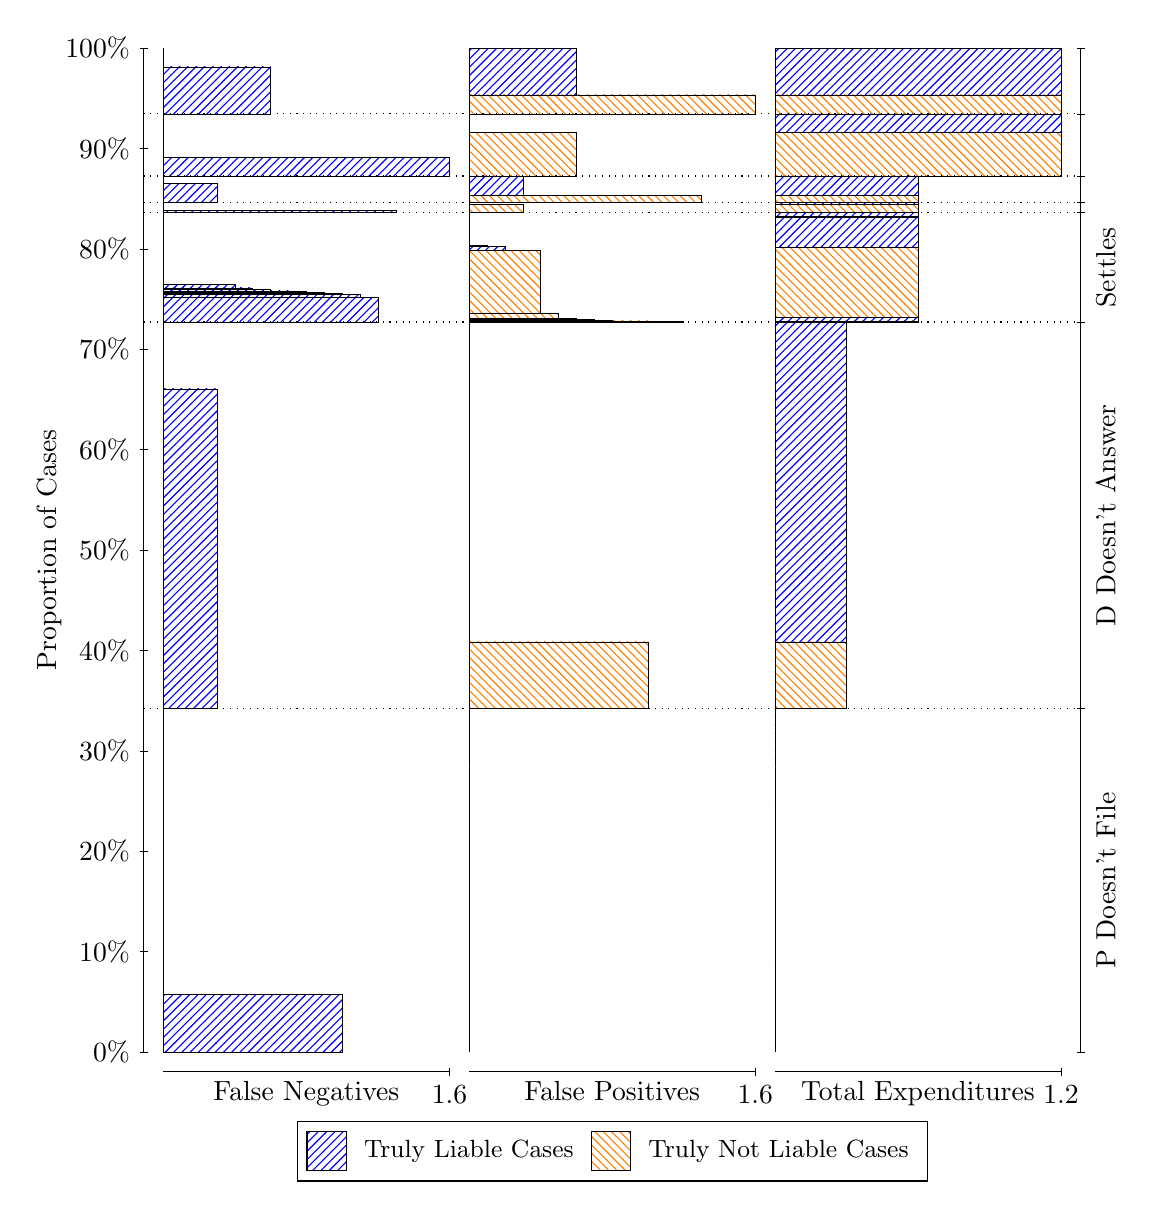
\begin{tikzpicture}
\draw[black, very thin] (1.5,1.75) -- (1.5,14.5);
\node[rotate=90, anchor=center] at (0.3, 8.125) {Proportion of Cases};
\draw[black, very thin] (1.45,1.75) -- (1.55,1.75);
\node[anchor=east] at (1.45, 1.75) {0\%};
\draw[black, very thin] (1.45,3.025) -- (1.55,3.025);
\node[anchor=east] at (1.45, 3.025) {10\%};
\draw[black, very thin] (1.45,4.3) -- (1.55,4.3);
\node[anchor=east] at (1.45, 4.3) {20\%};
\draw[black, very thin] (1.45,5.575) -- (1.55,5.575);
\node[anchor=east] at (1.45, 5.575) {30\%};
\draw[black, very thin] (1.45,6.85) -- (1.55,6.85);
\node[anchor=east] at (1.45, 6.85) {40\%};
\draw[black, very thin] (1.45,8.125) -- (1.55,8.125);
\node[anchor=east] at (1.45, 8.125) {50\%};
\draw[black, very thin] (1.45,9.4) -- (1.55,9.4);
\node[anchor=east] at (1.45, 9.4) {60\%};
\draw[black, very thin] (1.45,10.675) -- (1.55,10.675);
\node[anchor=east] at (1.45, 10.675) {70\%};
\draw[black, very thin] (1.45,11.95) -- (1.55,11.95);
\node[anchor=east] at (1.45, 11.95) {80\%};
\draw[black, very thin] (1.45,13.225) -- (1.55,13.225);
\node[anchor=east] at (1.45, 13.225) {90\%};
\draw[black, very thin] (1.45,14.5) -- (1.55,14.5);
\node[anchor=east] at (1.45, 14.5) {100\%};

\draw[black, very thin] (13.4,1.75) -- (13.4,14.5);
\draw[black, very thin] (13.35,1.75) -- (13.45,1.75);
\node[anchor=west] at (13.35, 1.75) {};
\draw[black, very thin] (13.35,6.1089) -- (13.45,6.1089);
\node[anchor=west] at (13.35, 6.1089) {};
\draw[black, very thin] (13.35,11.02) -- (13.45,11.02);
\node[anchor=west] at (13.35, 11.02) {};
\draw[black, very thin] (13.35,12.409) -- (13.45,12.409);
\node[anchor=west] at (13.35, 12.409) {};
\draw[black, very thin] (13.35,12.54) -- (13.45,12.54);
\node[anchor=west] at (13.35, 12.54) {};
\draw[black, very thin] (13.35,12.875) -- (13.45,12.875);
\node[anchor=west] at (13.35, 12.875) {};
\draw[black, very thin] (13.35,13.665) -- (13.45,13.665);
\node[anchor=west] at (13.35, 13.665) {};
\draw[black, very thin] (13.35,14.5) -- (13.45,14.5);
\node[anchor=west] at (13.35, 14.5) {};

\draw[black, very thin, pattern color=blue, pattern=north east lines] (1.75,1.75) rectangle (4.0208,2.4807);
\draw[black, very thin, pattern color=orange, pattern=north west lines] (1.75,2.4807) rectangle (1.75,6.1089);
\draw[black, very thin, pattern color=blue, pattern=north east lines] (1.75,6.1089) rectangle (2.4312,10.17);
\draw[black, very thin, pattern color=orange, pattern=north west lines] (1.75,10.17) rectangle (1.75,11.02);
\draw[black, very thin, pattern color=blue, pattern=north east lines] (1.75,11.02) rectangle (4.475,11.336);
\draw[black, very thin, pattern color=blue, pattern=north east lines] (1.75,11.336) rectangle (4.2479,11.368);
\draw[black, very thin, pattern color=blue, pattern=north east lines] (1.75,11.368) rectangle (4.0208,11.382);
\draw[black, very thin, pattern color=blue, pattern=north east lines] (1.75,11.382) rectangle (3.7937,11.396);
\draw[black, very thin, pattern color=blue, pattern=north east lines] (1.75,11.396) rectangle (3.7937,11.398);
\draw[black, very thin, pattern color=blue, pattern=north east lines] (1.75,11.398) rectangle (3.5667,11.411);
\draw[black, very thin, pattern color=blue, pattern=north east lines] (1.75,11.411) rectangle (3.3396,11.416);
\draw[black, very thin, pattern color=blue, pattern=north east lines] (1.75,11.416) rectangle (3.1125,11.438);
\draw[black, very thin, pattern color=blue, pattern=north east lines] (1.75,11.438) rectangle (2.8854,11.453);
\draw[black, very thin, pattern color=blue, pattern=north east lines] (1.75,11.453) rectangle (2.6583,11.496);
\draw[black, very thin, pattern color=orange, pattern=north west lines] (1.75,11.496) rectangle (1.75,12.409);
\draw[black, very thin, pattern color=blue, pattern=north east lines] (1.75,12.409) rectangle (4.7021,12.437);
\draw[black, very thin, pattern color=orange, pattern=north west lines] (1.75,12.437) rectangle (1.75,12.54);
\draw[black, very thin, pattern color=blue, pattern=north east lines] (1.75,12.54) rectangle (2.4312,12.785);
\draw[black, very thin, pattern color=orange, pattern=north west lines] (1.75,12.785) rectangle (1.75,12.875);
\draw[black, very thin, pattern color=blue, pattern=north east lines] (1.75,12.875) rectangle (5.3833,13.114);
\draw[black, very thin, pattern color=orange, pattern=north west lines] (1.75,13.114) rectangle (1.75,13.665);
\draw[black, very thin, pattern color=blue, pattern=north east lines] (1.75,13.665) rectangle (3.1125,14.26);
\draw[black, very thin, pattern color=orange, pattern=north west lines] (1.75,14.26) rectangle (1.75,14.5);
\draw[black, very thin, pattern color=orange, pattern=north west lines] (5.6333,1.75) rectangle (5.6333,5.3782);
\draw[black, very thin, pattern color=blue, pattern=north east lines] (5.6333,5.3782) rectangle (5.6333,6.1089);
\draw[black, very thin, pattern color=orange, pattern=north west lines] (5.6333,6.1089) rectangle (7.9042,6.9593);
\draw[black, very thin, pattern color=blue, pattern=north east lines] (5.6333,6.9593) rectangle (5.6333,11.02);
\draw[black, very thin, pattern color=orange, pattern=north west lines] (5.6333,11.02) rectangle (8.3583,11.026);
\draw[black, very thin, pattern color=orange, pattern=north west lines] (5.6333,11.026) rectangle (8.1313,11.028);
\draw[black, very thin, pattern color=orange, pattern=north west lines] (5.6333,11.028) rectangle (7.9042,11.034);
\draw[black, very thin, pattern color=orange, pattern=north west lines] (5.6333,11.034) rectangle (7.6771,11.036);
\draw[black, very thin, pattern color=orange, pattern=north west lines] (5.6333,11.036) rectangle (7.45,11.041);
\draw[black, very thin, pattern color=orange, pattern=north west lines] (5.6333,11.041) rectangle (7.2229,11.052);
\draw[black, very thin, pattern color=orange, pattern=north west lines] (5.6333,11.052) rectangle (6.9958,11.066);
\draw[black, very thin, pattern color=orange, pattern=north west lines] (5.6333,11.066) rectangle (6.7687,11.132);
\draw[black, very thin, pattern color=orange, pattern=north west lines] (5.6333,11.132) rectangle (6.5417,11.933);
\draw[black, very thin, pattern color=blue, pattern=north east lines] (5.6333,11.933) rectangle (6.0875,11.976);
\draw[black, very thin, pattern color=blue, pattern=north east lines] (5.6333,11.976) rectangle (5.8604,11.991);
\draw[black, very thin, pattern color=blue, pattern=north east lines] (5.6333,11.991) rectangle (5.6333,12.409);
\draw[black, very thin, pattern color=orange, pattern=north west lines] (5.6333,12.409) rectangle (6.3146,12.512);
\draw[black, very thin, pattern color=blue, pattern=north east lines] (5.6333,12.512) rectangle (5.6333,12.54);
\draw[black, very thin, pattern color=orange, pattern=north west lines] (5.6333,12.54) rectangle (8.5854,12.63);
\draw[black, very thin, pattern color=blue, pattern=north east lines] (5.6333,12.63) rectangle (6.3146,12.875);
\draw[black, very thin, pattern color=orange, pattern=north west lines] (5.6333,12.875) rectangle (6.9958,13.426);
\draw[black, very thin, pattern color=blue, pattern=north east lines] (5.6333,13.426) rectangle (5.6333,13.665);
\draw[black, very thin, pattern color=orange, pattern=north west lines] (5.6333,13.665) rectangle (9.2667,13.905);
\draw[black, very thin, pattern color=blue, pattern=north east lines] (5.6333,13.905) rectangle (6.9958,14.5);
\draw[black, very thin, pattern color=orange, pattern=north west lines] (9.5167,1.75) rectangle (9.5167,5.3782);
\draw[black, very thin, pattern color=blue, pattern=north east lines] (9.5167,5.3782) rectangle (9.5167,6.1089);
\draw[black, very thin, pattern color=orange, pattern=north west lines] (9.5167,6.1089) rectangle (10.425,6.9593);
\draw[black, very thin, pattern color=blue, pattern=north east lines] (9.5167,6.9593) rectangle (10.425,11.02);
\draw[black, very thin, pattern color=orange, pattern=north west lines] (9.5167,11.02) rectangle (11.333,11.034);
\draw[black, very thin, pattern color=blue, pattern=north east lines] (9.5167,11.034) rectangle (11.333,11.084);
\draw[black, very thin, pattern color=orange, pattern=north west lines] (9.5167,11.084) rectangle (11.333,11.975);
\draw[black, very thin, pattern color=blue, pattern=north east lines] (9.5167,11.975) rectangle (11.333,12.351);
\draw[black, very thin, pattern color=orange, pattern=north west lines] (9.5167,12.351) rectangle (11.333,12.359);
\draw[black, very thin, pattern color=blue, pattern=north east lines] (9.5167,12.359) rectangle (11.333,12.409);
\draw[black, very thin, pattern color=orange, pattern=north west lines] (9.5167,12.409) rectangle (11.333,12.512);
\draw[black, very thin, pattern color=blue, pattern=north east lines] (9.5167,12.512) rectangle (11.333,12.54);
\draw[black, very thin, pattern color=orange, pattern=north west lines] (9.5167,12.54) rectangle (11.333,12.63);
\draw[black, very thin, pattern color=blue, pattern=north east lines] (9.5167,12.63) rectangle (11.333,12.875);
\draw[black, very thin, pattern color=orange, pattern=north west lines] (9.5167,12.875) rectangle (13.15,13.426);
\draw[black, very thin, pattern color=blue, pattern=north east lines] (9.5167,13.426) rectangle (13.15,13.665);
\draw[black, very thin, pattern color=orange, pattern=north west lines] (9.5167,13.665) rectangle (13.15,13.905);
\draw[black, very thin, pattern color=blue, pattern=north east lines] (9.5167,13.905) rectangle (13.15,14.5);
\draw[black, dotted] (1.5,6.1089) -- (13.4,6.1089);
\draw[black, dotted] (1.5,11.02) -- (13.4,11.02);
\draw[black, dotted] (1.5,12.409) -- (13.4,12.409);
\draw[black, dotted] (1.5,12.54) -- (13.4,12.54);
\draw[black, dotted] (1.5,12.875) -- (13.4,12.875);
\draw[black, dotted] (1.5,13.665) -- (13.4,13.665);
\draw[black, very thin] (1.75,1.5) -- (5.3833,1.5);
\node[anchor=north] at (3.5667, 1.5) {False Negatives};
\draw[black, very thin] (5.3833,1.45) -- (5.3833,1.55);
\node[anchor=north] at (5.3833, 1.45) {1.6};

\draw[black, very thin] (5.6333,1.5) -- (9.2667,1.5);
\node[anchor=north] at (7.45, 1.5) {False Positives};
\draw[black, very thin] (9.2667,1.45) -- (9.2667,1.55);
\node[anchor=north] at (9.2667, 1.45) {1.6};

\draw[black, very thin] (9.5167,1.5) -- (13.15,1.5);
\node[anchor=north] at (11.333, 1.5) {Total Expenditures};
\draw[black, very thin] (13.15,1.45) -- (13.15,1.55);
\node[anchor=north] at (13.15, 1.45) {1.2};

\node[black, centered, rotate=90] at (13.72, 3.9295) {P Doesn't File};
\node[black, centered, rotate=90] at (13.72, 8.5645) {D Doesn't Answer};
\node[black, centered, rotate=90] at (13.72, 11.715) {Settles};





\draw (7.449999999999999,1.5) node[draw=none] (baseCoordinate) {};
\begin{scope}[align=center]
        \matrix[scale=0.5, draw=black, below=0.5cm of baseCoordinate, nodes={draw}, column sep=0.1cm]{
            \node[rectangle, draw, minimum width=0.5cm, minimum height=0.5cm, pattern=north east lines, pattern color=blue] {}; &
            \node[draw=none, font=\small] (B) {Truly Liable Cases}; &
            \node[rectangle, draw, minimum width=0.5cm, minimum height=0.5cm, pattern=north west lines, pattern color=orange] {}; &
            \node[draw=none, font=\small] (B) {Truly Not Liable Cases}; \\
            };
\end{scope}

\end{tikzpicture}
\end{document}